\documentclass[a4paper,10pt]{article}
\usepackage[utf8x]{inputenc}
\usepackage{listings}
\usepackage{a4wide}
\usepackage{tabularx}
\usepackage{booktabs}
\usepackage{graphicx}

\lstloadlanguages{Bash}
\lstset{basicstyle=\small\ttfamily, escapeinside={(*@}{@*)},
showstringspaces=false, breaklines=true, breakatwhitespace=true,
tabsize=4, language=Bash, numberfirstline=true,
commentstyle=\itshape\color{CommentGreen},
stringstyle=\color{DataTypeBlue}}
\newcommand{\ilcode}[1]{\lstinline|#1|}

\title{RTC:PCL User Guide}
\author{Geoffrey Biggs}

\begin{document}
\maketitle

\setcounter{tocdepth}{1}
\tableofcontents

\newpage

\section{Introduction}
\label{sec:intro}

RTC:PCL is a library of components for working with point clouds. It uses the
PCL library\footnote{http://www.pointclouds.org} for data capture, processing
and visualisation.

This software is developed at the National Institute of Advanced Industrial
Science and Technology. Approval number H23PRO-1298. This software is licensed
under the Lesser General Public License. See COPYING and COPYING.LESSER in the
source.

\section{Requirements}
\label{sec:requirements}

RTC:PCL requires the C++ version of OpenRTM-aist-1.0.0.

RTC:PCL uses the CMake build system\footnote{http://www.cmake.org/}. You will
need at least version 2.6 to be able to build the component.

RTC:PCL requires PCL version 1.1.

RTC:PCL can optionally take advantage of the RTM:DDS transport. If it is
installed, you can compile the components with DDS support by enabling the
\verb|DDS_SUPPORT| option in CMake.

\section{Installation}
\label{sec:installation}

\subsection{Binary}

Users of Windows can install the components using the binary installer. This
will install the components and all necessary dependencies. It is the
recommended method of installation in Windows.

\begin{enumerate}
  \item Download the installer from the website.
  \item Double-click the executable file to begin installation.
  \item Follow the instructions to install the component.
  \item You may need to restart your computer for environment variable changes
  to take effect before using the component.
\end{enumerate}

The components can be launched by double-clicking the relevant executables. For
example, \verb|rtc_pclviewer_standalone| will launch the cloud viewer
component. Each component is also available as a shared library that can be
loaded into a manager. The initialisation function for each component is
\verb|rtc_init|.

\subsection{From source}

Follow these steps to install :

\begin{enumerate}
  \item Download the source, either from the repository or a source archive,
  and extract it somewhere.

  \verb|tar -xvzf rtcpcl.tar.gz|
  \item Change to the directory containing the extracted source.

  \verb|cd rtcpcl-1.0.0|
  \item Create a directory called ``build'':

  \verb|mkdir build|
  \item Change to that directory.

  \verb|cd build|
  \item Run cmake or cmake-gui.

  \verb|cmake ../|
  \item If no errors occurred, run make.

  \verb|make|
  \item Finally, install the components. Ensure the necessary permissions to
  install into the chosen prefix are available.

  \verb|make install|
  \item The install destination can be changed by executing ccmake and changing
  the variable \verb|CMAKE_INSTALL_PREFIX|.

  \verb|ccmake ../|
\end{enumerate}

The components are now ready for use. See the next sections for instructions on
configuring each components.

RTC:PCL components can be launched in stand-alone mode by executing the
appropriate \verb|*_standalone| executable (installed into
\verb|${prefix}/bin|). Alternatively, \verb|librtc*.so| can be loaded into a
manager, using the initialisation function \verb|rtc_init|. This shared objects
can be found in \verb|${prefix}/lib| or \verb|${prefix}/lib64|.


\section{Common Configuration}
\label{sec:common_configuration}

Some configuration parameters are common across all components in RTC:PCL.
These are described in Table~\ref{tab:common_config_params}.

\begin{table}[t]
  \centering
  \begin{tabularx}{\columnwidth}{lX}
    \toprule
    Parameter & Effect \\
    \midrule
    corba & Enable input/output of data on the DataPort ports (typically using the CORBA transport). \\
    dds & Enable input/output of data on the DDSPort ports. DDS support must have been compiled in and the RTM:DDS transport must be available. \\
    pointer & Enable input/output of data on the PointerPort ports. PointerPort support must have been compiled in and the RTM:Pointer transport must be available. [Not implemented.] \\
    \bottomrule
  \end{tabularx}
  \caption{Common configuration parameters.}
  \label{tab:common_config_params}
\end{table}

Each port in each component is duplicated for each transport that was enabled
at compile time. This means that, for example, if you compiled with both CORBA
and DDS support, you will get two of every port; one for each transport type.
These ports are prefixed with the name of the transport they correspond to.

\section{RTCPCLViewer}
\label{sec:rtcpclviewer}

RTCPCLViewer is a component for visualising point clouds. It can visualise
virtually any point cloud that PCL's visualiser can handle. It is capable of
visualising multiple point clouds, either in a single viewport or in separate
viewports. The input ports are configured at activation-time based on the value
of the \verb|ports| configuration parameter.

\begin{figure}
  \centering
  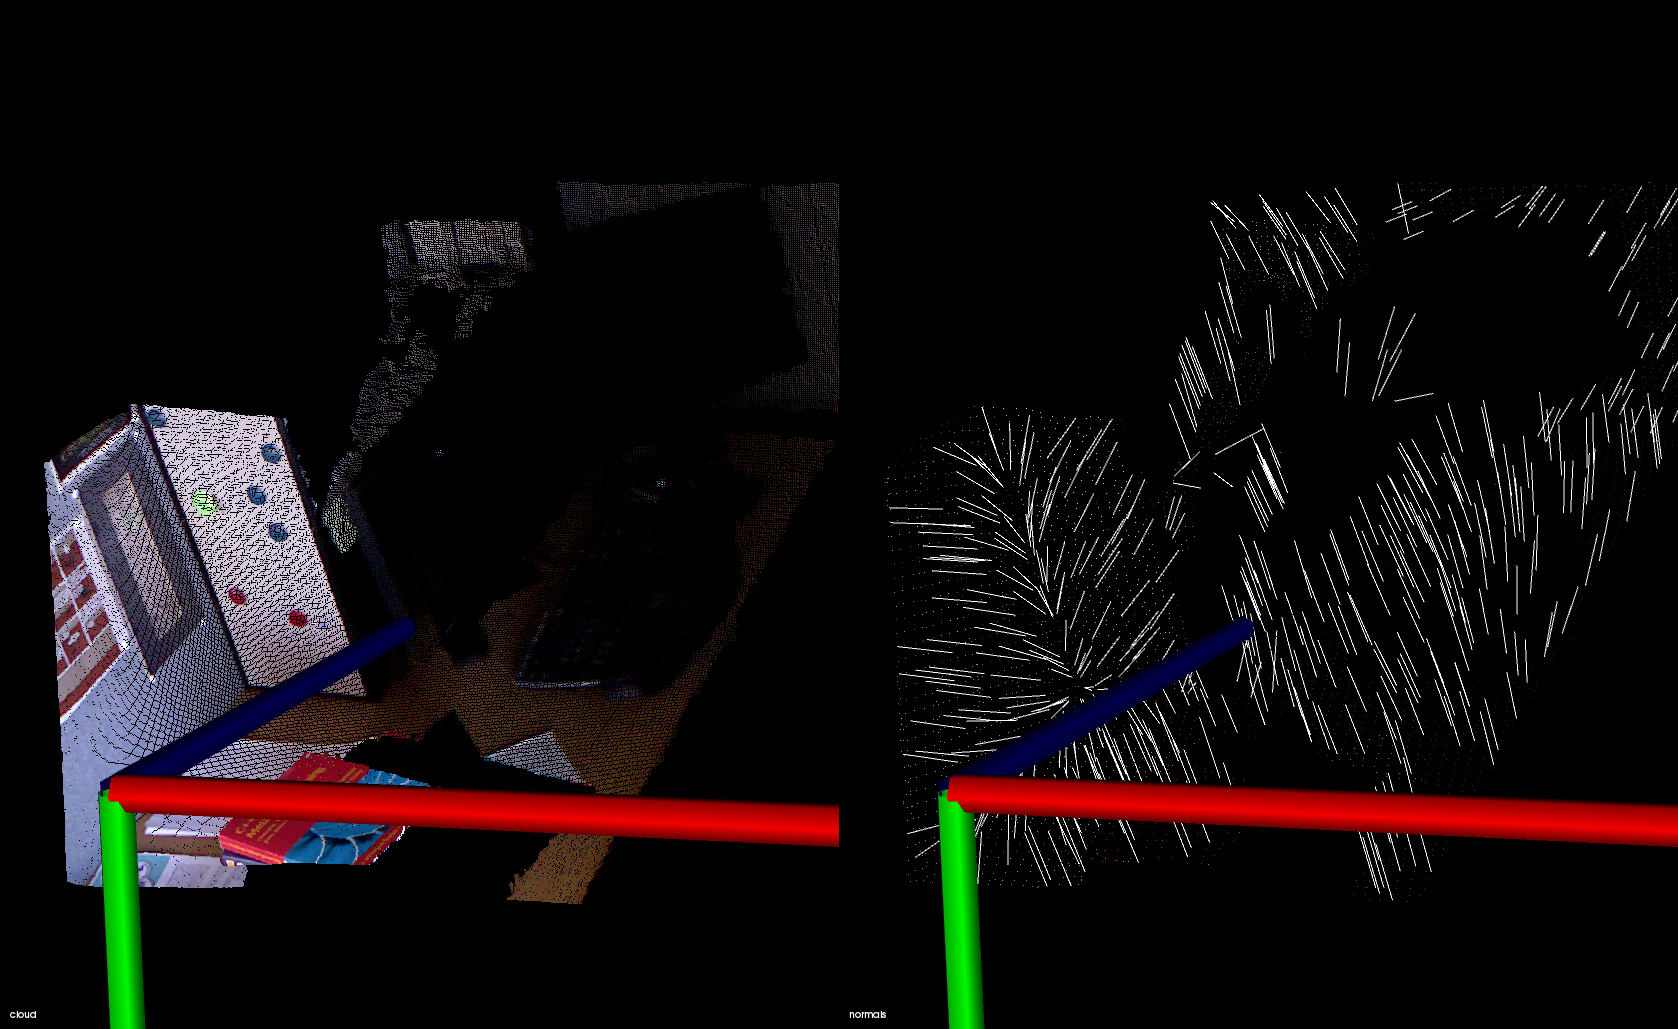
\includegraphics[width=\columnwidth,keepaspectratio]{rtcpclviewer_normals_large}
  \caption{RTCPCLViewer showing a point cloud on the left and its normals on the right.}
  \label{fig:rtcpclviewer}
\end{figure}

\subsection{Configuration}
\label{sec1:viewer_configuration}

The available configuration parameters are described in
Table~\ref{tab:viewer_config_params}.

\begin{table}[t]
  \centering
  \begin{tabularx}{\columnwidth}{lX}
    \toprule
    Parameter & Effect \\
    \midrule
    axes\_scale & Set the scale of the axes displayed in the viewports. Set to 0 to disable. \\
    ports & Set the ports that the component will provide, including how the received data is displayed. \\
    show\_timestamps & Print timestamps for the received data in the terminal. Useful for checking the lag of the visualisation. \\
    \bottomrule
  \end{tabularx}
  \caption{Available configuration parameters for RTCPCLViewer.}
  \label{tab:viewer_config_params}
\end{table}

\subsection{Ports}
\label{sec1:viewer_port}

RTCPCLViewer does not provide any ports by default. You must set the \verb|ports| configuration parameter to get the the ports you require.

The format of the \verb|ports| parameter is:

\verb+name:viewport:type:colour,...+

where:

\begin{description}
  \item[name] Name of the port.
  \item[viewport] Viewport number. Set to 0 to display in all viewports.
  \item[type] The display type for the cloud. One of ``p'' (plain point cloud),
  ``n;x;y'' (normals, where ``x'' must be an integer giving the normals level
  and y must be a floating point number giving the normals scale), or ``c;x;y''
  (principal curvatures, where x and y have the same meaning as for normals).
  \item[colour] The colourisation method for the cloud. One of ``p'' for none,
  ``a'' for random, ``r'' for using the cloud's RGB data, ``x.y.z'', where x, y
  and z are integers between 0 and 255 depicting red, green and blue colour
  levels, for a custom colour, and ``"x"'', where ``x'' is a field name, for
  using a custom field for colourisation.
\end{description}

Apart from the name, any parameter may be left black to get the default.
Multiple port specifications should be separated by commas. For example, the
following string creates three ports. The first, named ``pc1'', is a plain
point cloud with RGB data, which it is using for colourisation. It is displayed
in viewport 1. The second, ``pc2'', contains normals information. It is
displayed in all viewports with a random colour. The third, named ``pc2'', is
another plain point cloud. It is displayed in viewport 3 using a custom colour
(green).

\verb|pc1:1:p:r,pc2::n;10;0.1:a,pc3:3:p:0.255.0|

\section{RTCRIViewer}
\label{sec:rtcriviewer}

RTCRIViewer is the range image equivalent of RTCPCLViewer. It is used to
visualise range images. These are point clouds where each three-dimensional
point corresponds to a pixel in a two-dimensional image.

\subsection{Configuration}
\label{sec1:riviewer_configuration}

The available configuration parameters are described in
Table~\ref{tab:riviewer_config_params}.

\begin{table}[t]
  \centering
  \begin{tabularx}{\columnwidth}{lX}
    \toprule
    Parameter & Effect \\
    \midrule
    unseen\_to\_max & When enabled, unseen pixels will be displayed in the colour for the maximum distance. \\
    \bottomrule
  \end{tabularx}
  \caption{Available configuration parameters for RTCRIViewer.}
  \label{tab:riviewer_config_params}
\end{table}

\subsection{Ports}
\label{sec1:riviewer_port}

The ports provided by the RTCRIViewer component are described in Table~\ref{tab:riviewer_ports}.

\begin{table}[t]
  \centering
  \begin{tabularx}{\columnwidth}{lllX}
    \toprule
    Name & Type & Data type & Purpose \\
    \midrule
    ri & Input & PointCloud & Receives the range-image-organised point cloud to display. \\
    \bottomrule
  \end{tabularx}
  \caption{Available ports for the RTCRIViewer component.}
  \label{tab:riviewer_ports}
\end{table}

\section{RTCPCLOpenNI}
\label{sec:rtcpclopenni}

RTCPCLOpenNI provides an input component for reading from OpenNI-compatible
depth cameras, such as the Microsoft Kinect. It can provide the data as a point
cloud or a range image.

\subsection{Configuration}
\label{sec1:openni_configuration}

The available configuration parameters are described in
Table~\ref{tab:openni_config_params}.

\begin{table}[t]
  \centering
  \begin{tabularx}{\columnwidth}{lX}
    \toprule
    Parameter & Effect \\
    \midrule
    device & The device number to open. Must be the path to the device node, or the index of the device, such as ``\#1'' or ``\#2''. \\
    output\_xyz & Enable outputting a plain XYZ point cloud, with no colour information. \\
    output\_xyzrgb & Enable outputting an XYZRGB point cloud. \\
    output\_ri & Enable outputting a range image. \\
    \bottomrule
  \end{tabularx}
  \caption{Available configuration parameters for RTCPCL.}
  \label{tab:openni_config_params}
\end{table}

\subsection{Ports}
\label{sec1:openni_port}

The ports provided by the RTCPCLOpenNI component are described in Table~\ref{tab:openni_ports}.

\begin{table}[t]
  \centering
  \begin{tabularx}{\columnwidth}{lllX}
    \toprule
    Name & Type & Data type & Purpose \\
    \midrule
    xyz & Output & PointCloud & Publishes the XYZ point cloud. \\
    xyzrgb & Output & PointCloud & Publishes the XYZRGB point cloud. \\
    ri & Output & PointCloud & Publishes the range image. \\
    \bottomrule
  \end{tabularx}
  \caption{Available ports on the RTCPCLOpenNI.}
  \label{tab:openni_ports}
\end{table}

\section{RTCPCDLoad}
\label{sec:rtcpcdload}

RTCPCDLoad loads point clouds stored in PCD files and sends them over its
output port. It is useful for replaying a previously-captured and saved (such
as with RTCPCDSave) point clouds.

\subsection{Configuration}
\label{sec1:pcdload_configuration}

The available configuration parameters are described in
Table~\ref{tab:pcdload_config_params}.

\begin{table}[t]
  \centering
  \begin{tabularx}{\columnwidth}{lX}
    \toprule
    Parameter & Effect \\
    \midrule
    write\_once & Only write the point cloud once. When disabled, the point cloud will be written every time the component executes. \\
    pcd\_file & File name of the PCD file to load the point cloud from. \\
    point\_type & The type of point used by the cloud stored in the PCD file. \\
    \bottomrule
  \end{tabularx}
  \caption{Available configuration parameters for RTCPCDLoad.}
  \label{tab:pcdload_config_params}
\end{table}

\subsection{Ports}
\label{sec1:pcdload_port}

The ports provided by the RTCPCDLoad component are described in Table~\ref{tab:pcdload_ports}.

\begin{table}[t]
  \centering
  \begin{tabularx}{\columnwidth}{lllX}
    \toprule
    Name & Type & Data type & Purpose \\
    \midrule
    out & Output & PointCloud & The point cloud loaded from the PCD file. \\
    \bottomrule
  \end{tabularx}
  \caption{Available ports on the RTCPCDLoad component.}
  \label{tab:pcdload_ports}
\end{table}

\section{RTCPCDSave}
\label{sec:rtcpcdsave}

RTCPCDSave performs the opposite function of RTCPCDLoad. It saves a received
point cloud into a PCD file.

\subsection{Configuration}
\label{sec1:pcdsave_configuration}

The available configuration parameters are described in
Table~\ref{tab:pcdsave_config_params}.

\begin{table}[t]
  \centering
  \begin{tabularx}{\columnwidth}{lX}
    \toprule
    Parameter & Effect \\
    \midrule
    binary & Save the point cloud in binary format instead of ASCII format. \\
    write\_once & Only save the first point cloud received. When disabled, every point cloud received will be saved, overwriting the previous point cloud. \\
    pcd\_file & File name of the PCD file to save the point cloud into. \\
    \bottomrule
  \end{tabularx}
  \caption{Available configuration parameters for RTCPCDSave.}
  \label{tab:pcdsave_config_params}
\end{table}

\subsection{Ports}
\label{sec1:pcdsave_port}

The ports provided by the RTCPCDSave component are described in Table~\ref{tab:pcdsave_ports}.

\begin{table}[t]
  \centering
  \begin{tabularx}{\columnwidth}{lllX}
    \toprule
    Name & Type & Data type & Purpose \\
    \midrule
    in & Input & PointCloud & Receives the point cloud to save. \\
    \bottomrule
  \end{tabularx}
  \caption{Available ports on the RTCPCDSave component.}
  \label{tab:pcdsave_ports}
\end{table}

\section{RTCPCLCuboid}
\label{sec:rtcpclcuboid}

This component generates a random point cloud where all points fit within a
cuboid. The dimensions of the cuboid and the number of points can be
configured. A new random point cloud is generated each time the component
executes.

\subsection{Configuration}
\label{sec1:cuboid_configuration}

The available configuration parameters are described in
Table~\ref{tab:cuboid_config_params}.

\begin{table}[t]
  \centering
  \begin{tabularx}{\columnwidth}{lX}
    \toprule
    Parameter & Effect \\
    \midrule
    count & Sets the number of points that will be generated. \\
    low\_x & The lower bound on the x-coordinate of the points. \\
    high\_x & The upper bound on the x-coordinate of the points. \\
    low\_y & The lower bound on the y-coordinate of the points. \\
    high\_y & The upper bound on the y-coordinate of the points. \\
    low\_z & The lower bound on the z-coordinate of the points. \\
    high\_z & The upper bound on the z-coordinate of the points. \\
    \bottomrule
  \end{tabularx}
  \caption{Available configuration parameters for RTCPCLCuboid.}
  \label{tab:cuboid_config_params}
\end{table}

\subsection{Ports}
\label{sec1:cuboid_port}

The ports provided by the RTCPCLCuboid component are described in
Table~\ref{tab:cuboid_ports}.

\begin{table}[t]
  \centering
  \begin{tabularx}{\columnwidth}{lllX}
    \toprule
    Name & Type & Data type & Purpose \\
    \midrule
    out & Output & PointCloud & Publishes the randomly-generated point cloud. \\
    \bottomrule
  \end{tabularx}
  \caption{Available ports on the RTCPCLCuboid component.}
  \label{tab:cuboid_ports}
\end{table}

\section{RTCPCLRainbowTube}
\label{sec:rtcpclrainbowtube}

Like RTCPCLCuboid, this component produces a sample point cloud. In this case, the point cloud is a tube of regularly-spaced points. The length of the major and minor axes, as well as the length of the overall tube, can be configured. The tube is coloured in RGB.

\subsection{Configuration}
\label{sec1:rainbowtube_configuration}

The available configuration parameters are described in
Table~\ref{tab:rainbowtube_config_params}.

\begin{table}[t]
  \centering
  \begin{tabularx}{\columnwidth}{lX}
    \toprule
    Parameter & Effect \\
    \midrule
    step & Sets the distance along the z-axis between each ring of points. \\
    angle\_step & Sets the angle around the z-axis between each column of points. \\
    x\_radius & Sets the length of the ellipsoid axis on the x-axis. \\
    y\_radius & Sets the length of the ellipsoid axis on the y-axis. \\
    length & Sets the length of the tube along the z-axis. \\
    \bottomrule
  \end{tabularx}
  \caption{Available configuration parameters for RTCPCLRainbowTube.}
  \label{tab:rainbowtube_config_params}
\end{table}

\subsection{Ports}
\label{sec1:cuboid_port}

The ports provided by the RTCPCLCuboid component are described in
Table~\ref{tab:cuboid_ports}.

\begin{table}[t]
  \centering
  \begin{tabularx}{\columnwidth}{lllX}
    \toprule
    Name & Type & Data type & Purpose \\
    \midrule
    out & Output & PointCloud & Publishes the randomly-generated point cloud. \\
    \bottomrule
  \end{tabularx}
  \caption{Available ports on the RTCPCLCuboid component.}
  \label{tab:cuboid_ports}
\end{table}

\section{RTCPCLVoxelFilter}
\label{sec:rtcpclvoxelfilter}

RTCPCLVoxel filter is a point cloud processing component. Its purpose is to
down-sample a point cloud, reducing the density of the points using a voxel
filter. Point clouds are often over-sampled when they come out of the sensor.
Passing them through a voxel filter can reduce the cloud complexity while
maintaining enough geometric accuracy for subsequent processing. This allows
those subsequent algorithms to execute much faster.

\subsection{Configuration}
\label{sec1:voxelfilter_configuration}

The available configuration parameters are described in
Table~\ref{tab:voxelfilter_config_params}.

\begin{table}[t]
  \centering
  \begin{tabularx}{\columnwidth}{lX}
    \toprule
    Parameter & Effect \\
    \midrule
    res\_x & Sets the x-axis resolution of the voxel grid. \\
    res\_y & Sets the y-axis resolution of the voxel grid. \\
    res\_z & Sets the z-axis resolution of the voxel grid. \\
    point\_type & Sets the point type to be filtered. For example, ``xyz'' or ``xyzrgb''. \\
    \bottomrule
  \end{tabularx}
  \caption{Available configuration parameters for RTCPCLVoxelFilter.}
  \label{tab:voxelfilter_config_params}
\end{table}

\subsection{Ports}
\label{sec1:voxelfilter_port}

The ports provided by the RTCPCLVoxelFilter component are described in Table~\ref{tab:voxelfilter_ports}.

\begin{table}[t]
  \centering
  \begin{tabularx}{\columnwidth}{lllX}
    \toprule
    Name & Type & Data type & Purpose \\
    \midrule
    in & Input & PointCloud & Receives the point cloud to be filtered. \\
    out & Output & PointCloud & Publishes the filtered point cloud. \\
    \bottomrule
  \end{tabularx}
  \caption{Available ports on the RTCPCLVoxelFilter component.}
  \label{tab:voxelfilter_ports}
\end{table}

\section{RTCPCLNormals}
\label{sec:rtcpclnormals}

RTCPCLNormals illustrates creating a component to deal with specific types of
point clouds. It takes in an XYZRGB point cloud, calculates the normal
information from the points, and outputs an XYZRGBNormal cloud containing both
the XYZ information and the Normal information. This cloud can be directly
displayed in RTCPCLViewer.

\subsection{Configuration}
\label{sec1:normals_configuration}

The available configuration parameters are described in
Table~\ref{tab:normals_config_params}.

\begin{table}[t]
  \centering
  \begin{tabularx}{\columnwidth}{lX}
    \toprule
    Parameter & Effect \\
    \midrule
    radius & Sets the search radius for finding neighbour points to calculate normals with. \\
    \bottomrule
  \end{tabularx}
  \caption{Available configuration parameters for RTCPCLNormals.}
  \label{tab:normals_config_params}
\end{table}

\subsection{Ports}
\label{sec1:normals_port}

The ports provided by the RTCPCLNormals component are described in Table~\ref{tab:normals_ports}.

\begin{table}[t]
  \centering
  \begin{tabularx}{\columnwidth}{lllX}
    \toprule
    Name & Type & Data type & Purpose \\
    \midrule
    in & Input & PointCloud (XYZRGB) & Receives the point cloud to be filtered. \\
    out & Output & PointCloud (XYZRGBNormal) & Publishes the filtered point cloud. \\
    \bottomrule
  \end{tabularx}
  \caption{Available ports on the RTCPCLNormals component.}
  \label{tab:normals_ports}
\end{table}

\section{RTCPCLBase}
\label{sec:rtcpcl}

RTCPCLBase is not a component in its own right. It is the base class used by
one-input, one-output processing components such as RTCPCLVoxelFilter.

The base class is available as a library installed by RTC:PCL. This library is
called \verb|rtcpclbase|, and the header file is \verb|rtcpclbase.h|. By
including this library, you can rapidly create new point cloud processing
components. For an example of using the library, see the source for the
RTCPCLVoxelFilter component.

\subsection{Configuration}
\label{sec1:_configuration}

RTCPCLBase does not provide any configuration parameters of its own.

\subsection{Ports}
\label{sec1:_port}

RTCPCLBase provides the ports described in Table~\ref{tab:base_ports}. These
are available for use by components that inherit from RTCPCLBase.

\begin{table}[t]
  \centering
  \begin{tabularx}{\columnwidth}{lllX}
    \toprule
    Name & Type & Data type & Purpose \\
    \midrule
    in & Input & PointCloud & Receives the point cloud to be processed. \\
    out & Output & PointCloud & Publishes the processed point cloud. \\
    \bottomrule
  \end{tabularx}
  \caption{Available ports on the RTCPCLBase component.}
  \label{tab:base_ports}
\end{table}

\section{PointCloud type}
\label{sec:pointcloud-type}

The PointCloud data type used by RTC:PCL to transport point clouds is defined
in \verb|pointcloud.idl|. This file is installed into
\verb|${prefix}/include/rtcpcl/idl|, so you can use it in your own components.
To make the use of this data type easier, RTC:PCL also installs a library
containing the data type compiled in each transport RTC:PCL is compiled to
support (by default, this is CORBA and DDS). By linking to this library, called
\verb|rtcpcl_pointcloud_type|, and including the appropriate headers for the
transports you want to use (such as \verb|pointcloud.hh| for the default CORBA
transport), you can immediately gain the use of this data type.

\section{Examples}
\label{sec:examples}

Example configuration files are provided in the
\verb|${prefix}/share/rtcpcl/examples/conf/| directory.

% \section{Changelog}


\end{document}
